\section{Comparação das Curvas à temperatura ambiente}
\label{sec:ResTAmb}

As medidas em temperatura ambiente foram realizadas no início de cada um dos ciclos de estresse (como indicado na Tabela \ref{tab:TempoDia}) antes de ligar a câmara térmica. As medidas apresentam uma certa oscilação devido a variabilidade da temperatura ambiente.

A Figura \ref{fig:TAmbEstressadas} mostra as curvas das frequências normalizadas dos osciladores das placas que foram estressadas em relação ao tempo de exposição. Nela é possível ver um comportamento da DE2 de uma diminuição da frequência no inicio dos ensaios seguido de uma estabilidade. Já a ZedBoard apresentou uma degradação maior e ao longo de todas as medidas, o formato da curva é o esperado segundo a Equação \ref{eq:VthTempo} que indica uma degradação decrescente.

\begin{figure}[H]
    \centering
    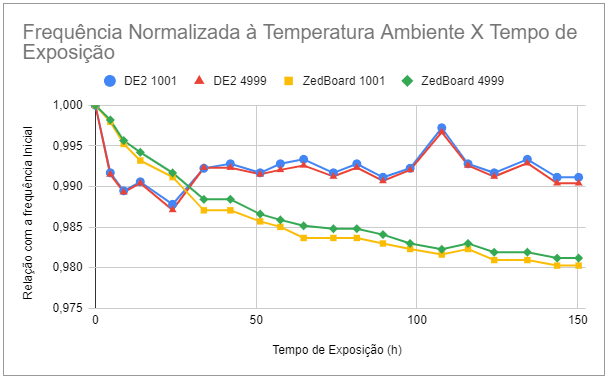
\includegraphics[scale=0.75]{figures/Resultados/TAmbEstressadas}
    \caption{Comparação das duas placas à temperatura ambiente. Fonte: O Autor}
    \label{fig:TAmbEstressadas}
\end{figure}

A Figura \ref{fig:TAmbDE2} mostra as curvas das frequências normalizadas dos osciladores das placas  DE2, tanto a que foi estressada termicamente quanto a que não foi estressada, em relação ao tempo de exposição.

É possível observar que a placa que não foi estressada apresenta uma curva semelhante à que foi estressada, o que pode indicar que o FPGA da DE2 não sofreu do NBTI e que a degradação é apenas decorrente do uso prolongado da placa ou que a temperatura não foi um fator tão relevante para o fenômeno, tendo sido, ambas as placas, afetados por ele da mesma forma.

\begin{figure}[H]
    \centering
    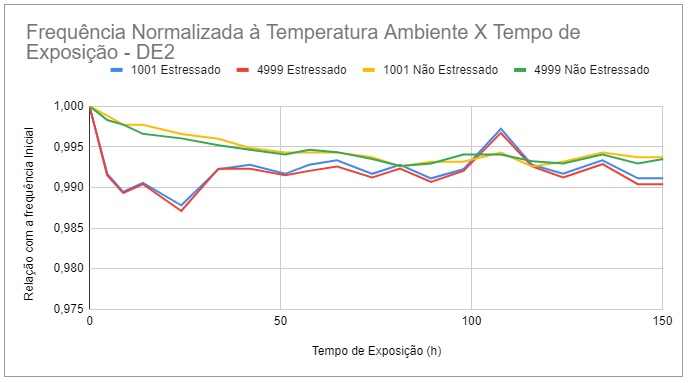
\includegraphics[scale=0.75]{figures/Resultados/TAmbDE2}
    \caption{Curva das placas DE2 à temperatura ambiente. Fonte: O Autor}
    \label{fig:TAmbDE2}
\end{figure}

As mesmas curvas são mostradas na Figura \ref{fig:TAmbZedBoard}, porém para as placas ZedBoard. Diferentemente da DE2, para a ZedBoard o comportamento entre a placa que foi estressada e a que não foi apresentaram uma diferença considerável, ambas possuem o mesmo formato porém a estressada demonstra uma queda maior na frequência.

\begin{figure}[H]
    \centering
    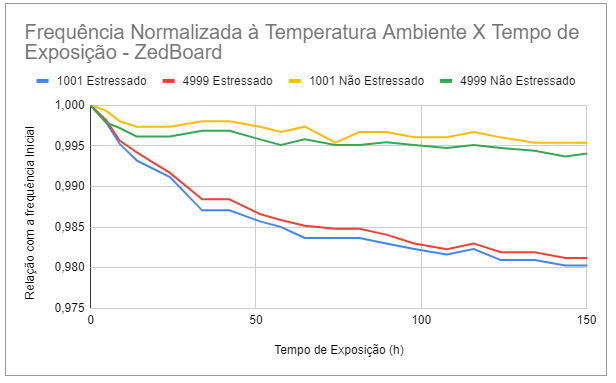
\includegraphics[scale=0.75]{figures/Resultados/TAmbZedBoard}
    \caption{Curva das placas DE2 a temperatura ambiente. Fonte: O Autor}
    \label{fig:TAmbZedBoard}
\end{figure}

A Tabela \ref{tab:FreqFinaisTAmb} mostra os valores finais das frequências de cada um dos osciladores. Já a Tabela \ref{tab:DegradFinaisTAmb} mostra a porcentagem da degradação das frequências em relação às frequências iniciais.

\begin{table}[H]
\centering
\caption{Frequências finais dos osciladores à temperatura ambiente.}
\begin{tabular}{l|cccc|}
\cline{2-5}
 & \multicolumn{4}{c|}{\textbf{Frequência (kHz)}} \\ \cline{2-5} 
 & \multicolumn{2}{c|}{\textbf{Altera DE2}} & \multicolumn{2}{c|}{\textbf{ZedBoard}} \\ \cline{2-5} 
 & \multicolumn{1}{c|}{\textbf{1001}} & \multicolumn{1}{c|}{\textbf{4999}} & \multicolumn{1}{c|}{\textbf{1001}} & \textbf{4999} \\ \hline
\multicolumn{1}{|l|}{\textbf{Estressados}} & \multicolumn{1}{c|}{1789} & \multicolumn{1}{c|}{361,4} & \multicolumn{1}{c|}{1441} & 271,3 \\ \hline
\multicolumn{1}{|l|}{\textbf{Não Estressados}} & \multicolumn{1}{c|}{1745} & \multicolumn{1}{c|}{352,2} & \multicolumn{1}{c|}{1513} & 284,3 \\ \hline
\end{tabular}
\label{tab:FreqFinaisTAmb}
\end{table}

\begin{table}[H]
\centering
\caption{Degradação na frequência dos osciladores à temperatura ambiente.}
\begin{tabular}{l|cr|cr|}
\cline{2-5}
 & \multicolumn{2}{c|}{\textbf{Altera DE2}} & \multicolumn{2}{c|}{\textbf{ZedBoard}} \\ \cline{2-5} 
 & \multicolumn{1}{c|}{\textbf{1001}} & \multicolumn{1}{c|}{\textbf{4999}} & \multicolumn{1}{c|}{\textbf{1001}} & \multicolumn{1}{c|}{\textbf{4999}} \\ \hline
\multicolumn{1}{|l|}{\textbf{Estressados}} & \multicolumn{1}{r|}{0,89\%} & 0,96\% & \multicolumn{1}{r|}{1,97\%} & 1,88\% \\ \hline
\multicolumn{1}{|l|}{\textbf{Não Estressados}} & \multicolumn{1}{r|}{0,63\%} & 0,65\% & \multicolumn{1}{r|}{0,46\%} & 0,59\% \\ \hline
\end{tabular}
\label{tab:DegradFinaisTAmb}
\end{table}

Na Tabela \ref{tab:DegradFinaisTAmb} é confirmado o que foi visto na Figura \ref{fig:TAmbEstressadas} de que a ZedBoard apresentou uma degradação maior que a DE2. Além disso, nela também é visível que a diferença entre o dispositivo estressado e o não estressado é consideravelmente maior no caso da ZedBoard do que no caso da DE2, corroborando com o mostrado nas Figuras \ref{fig:TAmbDE2} e \ref{fig:TAmbZedBoard}.

Um fato que ficou evidente aqui e se repetirá nas seções seguintes é que o comportamento dos osciladores de uma mesma placa, de 1001 e de 4999 inversores, foi semelhante.

Um problema encontrado nestas medidas foi, justamente, a variabilidade da temperatura ambiente, que, por ter influência no valor da frequência, causou um certo ruído nas medidas, principalmente nas da DE2 que foi estressada.